\chapter{Верификация выявленных звезд-кандидатов в двойные системы методом спекл-интерферометрии} \label{ch:ch5}
После выхода работы \cite{2015AstL...41..833K}, содержание которой было изложено во второй части предыдущей главы, возникла логичная необходимость верифицировать результаты, подтвердить двойственность исследуемых объектов. Cовместно с коллегами из САО РАН и ГАИШ МГУ была разработана методика дальнейших исследований. Предполагалось, что из списка полученных кандидатов в $\Delta\mu$-двойные будут отбираться звезды для спекл-интерферометрических исследований.
В первую заявку на спекл-наблюдения были включены 12 звезд из числа 144, выявленных астрометрически. Такие звезды характеризовались значительными величинами параметра F. Кроме того, спекл-наблюдения по понятным причинам ограничены по блеску. В окончательный список отбирались объекты до $13^m$ в полосе V.
 Наблюдения было решено проводить на телескопе БТА САО РАН и 2.5--метровом телескопе КГО ГАИШ МГУ. Уже в первой сессии спекл-исследований был получен  значимый результат, была подтверждена двойственность звезды J1158+4239. Статья с результатами исследований по этому объекту была опубликована в 2016 году \cite{2016AstL...42..686K}.
Звезда J1158+4239, имеющая блеск $12.09^m$ в полосе V, была одной из самых ярких в списке и потому наиболее перспективной. Компоненты ее собственного движения в каталоге LSPM составляют --330~mas/yr и 61~mas/yr по RA и Dec соответственно. В работе \cite{2011AstL...37..420K} ее квазимгновенное движение оказалось  $-303.3\pm 8.8$~mas/yr   $114.1\pm9.0$~mas/yr, что и обеспечило значение $F = 4.44$.

На рисунке~\ref{fig:J1158+4258_motion} показано движение фотоцентра системы J1158+4239. Для всех использованных обзоров (1995 "--- POSS1, 1984 "--- GSC1, 1990 и 1991 "--- POSS2, 1996 "--- GSC2, 2003 "--- SDSS, 2012 "--- пулковские наблюдения) удалось отобрать 8 опорных звезд, изображения которых надежно аппроксимируются на всех снимках с приемлемым значением отношения сигнал-шум. В результате для среднего движения фотоцентра по всем точкам компоненты собственного движения оказались $-326.4\pm1.7$~mas/yr и $50.1\pm7.1$~mas/yr. Для квазисреднего движения получилось $-335.9\pm6.4$~mas/yr и   $84.7\pm6.3$~mas/yr. Квазимгновенное собственное движение (2003 -- 2012) составило $-303.7\pm8.5$~mas/yr    и   $21.1\pm7.9$~mas/yr. Значение критерия $F = 6.99$, что не противоречит ранее сделанным оценкам (звезда может рассматриваться как кандидат в астрометрические двойные).

\begin{figure*}
\centering
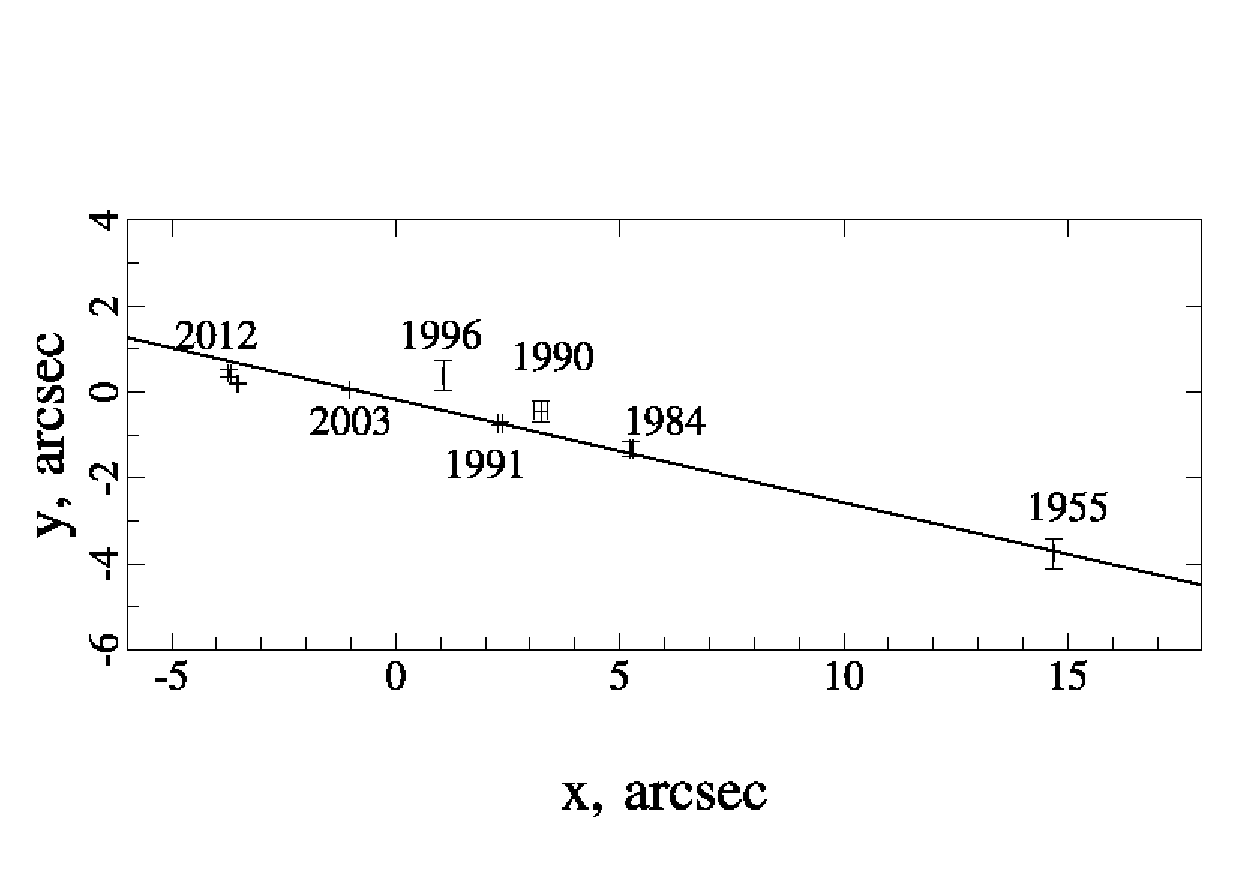
\includegraphics[width=0.95\columnwidth]{16fig2.eps}
%\setcaptionmargin{5mm}
%\captionstyle{normal}
\caption{Движение фотоцентра системы J1158+4239 по данным фотографических и цифровых обзоров неба (1955 "--- POSS1, 1984 "--- GSC1, 1990 и 1991 "--- POSS2, 1996 "--- GSC2, 2003 "--- SDSS, 2012 "--- пулковские наблюдения). Линия характеризует среднее движение фотоцентра.  Взято из работы \cite{2016AstL...42..686K}, рис. 2.}
\label{fig:J1158+4258_motion}
\end{figure*}
На БТА САО РАН для наблюдений использовалась  EMCCD--камера Andor iXon Ultra, а 2,5--метровый телескоп КГО ГАИШ МГУ оснащен спекл-поляриметром\footnote{\textit{http//lnfm1.sai.msu.ru/kgo/instruments/mfc/SPPdesign.pdf}}. Все наблюдения проводились в 2015--2016 гг.  Подробное описание спекл-наблюдений дано коллегами в нашей совместной работе \cite{2016AstL...42..686K}. В итоге наблюдений в САО РАН были получены позиционные параметры системы и разность блеска компонент (итоговые результаты представлены в таблице~\ref{tab:SI_meas}).  Примеры спекл-интерферограммы и восстановленного изображения представлены на рисунке~\ref{fig:sao_spekle_image}.

\begin{table}[p]
\centering
\caption{Спекл-интерферометрические измерения J1158+4239, выполненные на БТА САО РАН. Взято из работы \cite{2016AstL...42..686K}, таб. 1.}
\label{tab:SI_meas}
\bigskip
\begin{tabularx}{\textwidth}{l|l|ll|ll|ll}
Epoch      & $\lambda /\Delta \lambda, nm$ & $\Delta m$ & $\sigma _{\Delta m}$ & $\rho, mas$ & $\sigma _\rho$ & $\theta, \deg $& $\sigma_\theta$ \\
\hline
2015.43317 & 800/100 & 0.48 & 0.04 & 282 & 3  & 228.6 & 0.5               \\
2015.82798 & 800/100 & 0.54 & 0.03 & 284 & 1  & 230.2 & 0.1               \\
2015.97313 & 800/100 & 0.59 & 0.03 & 287 & 1  & 230.2 & 0.1               \\
2016.13692 & 800/100 & 0.70 & 0.08 & 288 & 1  & 230.9 & 0.2               \\
\hline
\end{tabularx}
\end{table}

\begin{figure}
\centering
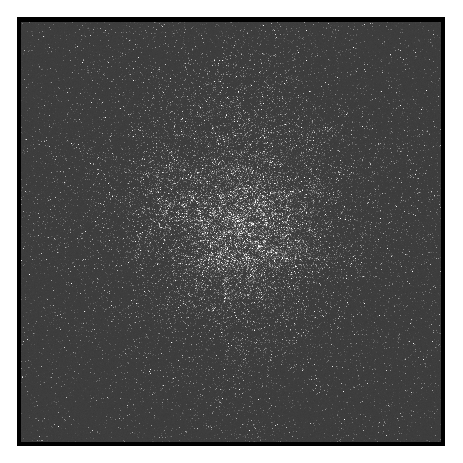
\includegraphics[width=0.445\columnwidth]{j1158plus4239_speckle_image.eps}
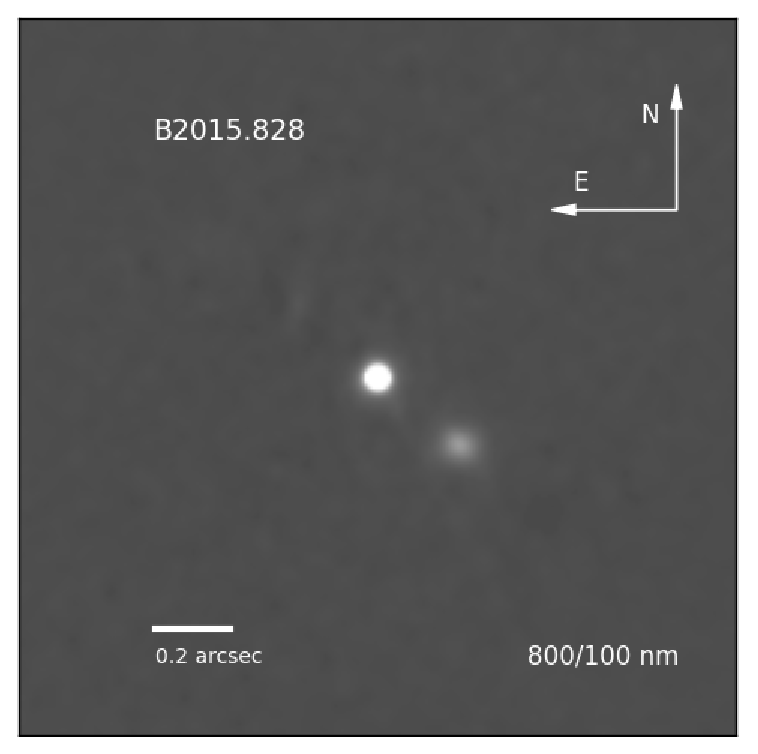
\includegraphics[width=0.45\columnwidth]{j1158plus4239_reconstructed_oct2015.eps}
%\setcaptionmargin{5mm}
%\captionstyle{normal}
\caption{Слева: спекл-интерферограмма J1158+4239, полученная на БТА САО РАН. Справа: соответствующее восстановленное изображение двойной системы J1158+4239. Взято из работы \cite{2016AstL...42..686K}, рис. 3.}
\label{fig:sao_spekle_image}
\end{figure}

Необходимо пояснить, что система J1158+4239 на момент публикации статьи отсутствовала в каталоге WDS и каких-либо доступных каталогах двойных звезд. То есть можно говорить о том, что данная звезда была детектирована нами как двойная впервые. Средневзвешенные оценки наблюдаемых параметров J1158+4239 на  эпоху B2015.88248 таковы: $\rho = 286.2\pm0.9$~mas и $\theta=230.24\pm0.16^\circ$. Разность блеска компонент, полученная на БТА САО РАН, составила $\Delta m = 0.55\pm0.03$ (фильтр 800/100~нм). Наблюдения, выполненные в КГО, дают $\Delta m = 0.9\pm0.1$ (фильтр $R$). Результаты определения астрометрических параметров БТА САО РАН и 2.5-метрового телескопа КГО находятся в хорошем согласии между собой.  

Сейчас ведутся дополнительные наблюдения данной системы с целью построения её орбиты. Предварительную орбиту можно увидеть на рисунке~\ref{fig:orbit}


\begin{figure}
\centering
\includegraphics[width=0.49\columnwidth]{orbitJ1158+4239}
\includegraphics[width=0.49\columnwidth]{orbitJ1158+4239_1}
\caption{Предварительная орбита J1158+4239, построенная по спекл-наблюдениями БТА САО РАН.}
\label{fig:orbit}
\end{figure}


Изображения остальных $\Delta\mu$-двойных долгое время не удавалось разделить на компоненты. Причиной может быть почти пороговое для спекл-интерферометрии значение блеска исследуемых звезд. В результате вторая компонента системы оказывалась за пределами возможностей метода. Тем не менее, после проведения спекл-сессии при более приемлемых погодных условиях звезда  J0259+3636 (см. рисунок~\ref{fig:j0259}) была разрешена. На данный момент есть автоковариационные функции (АКФ) этой звезды с интервалами более полугода. В обоих случаях уверенно регистрируется изображение второй компоненты, что исключает случайное наложение на звезду фона.

Стоит уточнить, что в программу спекл-наблюдений включаются всё новые объекты, и помимо кандидатов в $\Delta\mu$-двойные, проверке подлежат и объекты, выявленные в результате исследований форм изображений звезд, описанной в предыдущей главе. В настоящее время наблюдения проводились для 6 объектов из предложенного списка и среди них  4 объекта были детектированы как двойные. АКФ, иллюстрирующие двойственность объектов представлены далее. Помимо уже упомянутых J1158+4239 и J0259+3636, это  J1135+0414 (см. рисунок~\ref{fig:j1135}), J1147+6050 (см. рисунок~\ref{fig:j1147}), J1601+3714 (см. рисунок~\ref{fig:j1601}). Из них  J1601+3714, как и J0259+3636, включена в каталог WDS, и, помимо этого, также присутствует в 9-ом списке орбит спектроскопических двойных звезд \cite{2004A&A...424..727P}. Присутствие этих двух звезд в альтернативных перечнях двойных звезд может служить верификацией наших результатов. АФК J0259+3636 представлена на рисунке~\ref{fig:j0259}. Звезды J1135+0414 и J1147+6050 упоминаются как двойные только в рамках наших исследований. Наблюдения этих и других объектов продолжаются.

\begin{figure}[pt]
\centering
\includegraphics [scale=0.45] {j1135plus0414_acf_center}
\caption{Автоковариационная функция (АКФ) спекл-наблюдений звезды J1135+0414, проводимых на БТА САО РАН.}
\label{fig:j1135}
\end{figure}

\begin{figure}[pt]
\centering
\includegraphics [scale=0.45] {j1147plus6050_acf_center}
\caption{Автоковариационная функция (АКФ) спекл-наблюдений звезды J1147+6050, проводимых на БТА САО РАН.}
\label{fig:j1147}
\end{figure}

\begin{figure}[h]
\centering
\includegraphics [scale=0.45] {j1601plus3714_acf}
\caption{Автоковариационная функция (АКФ) спекл-наблюдений звезды J1601+3714, проводимых на БТА САО РАН. Вытянутость изображения спутника "--- эффект вращения поля зрения для альт-азимутального телескопа (по ряду причин не использовался ротатор поля).}
\label{fig:j1601}
\end{figure}

\begin{figure}[pt]
\centering
\includegraphics [scale=0.6] {J0259+3636}
\caption{Автоковариационная функция (АКФ) спекл-наблюдений звезды J0259+3636, проводимых на БТА САО РАН.}
\label{fig:j0259}
\end{figure}

Резюмируя этот короткий обзор спекл-наблюдений, отметим, что данную часть работы нельзя считать завершенной. Заявки на спекл-наблюдения регулярно подаются, но даже при их одобрении удается получить относительно небольшое количество наблюдательного времени (1--2 ночи в год). Тем не менее, продолжается проверка наших кандидатов в двойные системы, идет накопление рядов наблюдений для построения орбит уже подтвержденных двойных систем. 

В целом мы ожидали, что нам удастся подтвердить двойственность для большего количества кандидатов в $\Delta\mu$-двойные. На данном этапе можно выдвинуть несколько причин такого положения вещей. Как уже упоминалось, весьма вероятно, что изображение спутника имеет очень маленькое отношение сигнала к шуму. В ряде случаев наблюдения проводились в условиях, не самых благоприятных для выявления слабых объектов. Кроме того, изображения ярких звезд в обзорах POSS, SDSS близко к насыщению, выглядит асимметричным. Это могло привести к систематическим сдвигам в вычислении фотоцентров и к ошибочным определениям собственных движений.

В случае двойных систем, заподозренных методом анализа эллиптичности и асимметрии изображений, результативность ожидаемо более высокая. Дело в том, что для $\Delta\mu$-двойных невозможно заранее сказать, какой будет разность блеска компонент. Поэтому велик шанс <<не угадать>> с выбором объектов для спекл-наблюдений. Для звезд со значимой эллиптичностью есть гарантия, что разность блеска обычно не превышает $2^m$. 

В целом можно заключить, что применение разработанных в данном исследовании методик дает хорошую возможность сильно сузить круг поиска двойных систем среди близких карликов с помощью телескопов, оснащенных аппаратурой для применения различных методов высокого разрешения. В результате выявлены ранее неизвестные двойные системы, удобные для дальнейших исследований с целью построения орбит и оценки масс.
